\chapter{Thessa tool}
\section{Analysis on the Binomial filter algorithm}

The binomial filter implemented in this tools, is different from the one in this thesis.
The difference is that in this case it performs an arithmetic average as you can see above in C code
\lstset{ %Formatting for code in appendix
	language=C,
	basicstyle=\footnotesize,
	numbers=left,
	stepnumber=1,
	showstringspaces=false,
	tabsize=1,
	breaklines=true,
	breakatwhitespace=false,
}

\begin{lstlisting}[frame=single]  % Start your 

#include <stdio.h>
#define V 10000

int main(){
int w = 8;
int h = 8;
int in[h][w] = {{ 0,0,0,0,0,0,0,0},{ 0,1,6,6,1,1,1,0},{ 0,1,6,6,1,1,1,0},{ 0,1,6,6,1,1,1,0},{ 0,1,6,6,1,1,1,0},{ 0,1,6,6,1,1,6,0},{ 0,1,6,6,1,1,6,0},{ 0,0,0,0,0,0,0,0}};
int out[h][w];
int i;
int j;
int divisor = 8;

for (i = 1; i < h-1; i++){
for (j = 1; j < w-1; j=j+1){

out[i][j] = (in[i-1][j-1] + in[i-1][j] + in[i-1][j+1] + in[i][j-1] + in[i][j] + in[i][j+1] + in[i+1][j-1] + in[i+1][j] + in[i+1][j+1])/divisor;
}
}

return 0;
}
\end{lstlisting}
Having the C code, we have yo translate it in a lower language as the MiRcode and obtain the following code.

\begin{tabular}{l l l}
0   & &    ['\$s', 'i', '1'] \\
1     & &  ['+', '\_f1', 'i', '1']\\ 
2 & &      ['-', '\_f0', 'i', '1'] \\
3  & L3:& ['for', '$>$=', 'i', '7', 'goto', 'L0']\\ 
4 & &      ['\$s', 'j', '1'] \\
5    & &   ['+', '\_f3', 'j', '1'] \\
6       & &['-', '\_f2', 'j', '1'] \\
7   &L2:& ['for', '$>$=', 'j', '7', 'goto', 'L1'] \\
8   & &    ['+', '\_t0', 'in[i-1][j]', 'in[i-1][j-1]'] \\
9  & &     ['+', '\_t1', '\_t0', 'in[i-1][j+1]'] \\
10    & &  ['+', '\_t2', '\_t1', 'in[i][j-1]']\\
11& &   ['+', '\_t3', '\_t2', 'in[i][j]']\\
12& &   ['+', '\_t4', '\_t3', 'in[i][j+1]']\\
13& &   ['+', '\_t5', '\_t4', 'in[i+1][j-1]']\\
14& &   ['+', '\_t6', '\_t5', 'in[i+1][j]']\\
15 & &  ['+', '\_t7', '\_t6', 'in[i+1][j+1]']\\ 
16 & &  ['/', '\_t8', '\_t7', 'divisor'] \\
17 & &  ['\$s', 'out[i][j]', '\_t8'] \\
18 & &  ['+', '\_t9', 'j', '1'] \\
19 & &  ['\$s', 'j', '\_t9'] \\
20 & &  ['+', '\_f3', 'j', '1']\\
21 & &  ['-', '\_f2', 'j', '1'] \\
22 & &  ['goto', 'L2']
\end{tabular}\\

\begin{tabular}{l l l}
23  &L1:& ['+', '\_t10', 'i', '1']\\
24 & &  ['\$s', 'i', '\_t10'] \\
25 & &  ['+', '\_f1', 'i', '1']\\
26 & &  ['-', '\_f0', 'i', '1']\\
27 & &  ['goto', 'L3']\\
28  &L0:& ['\$s', 'reset', '0']\\

\end{tabular}\\

After that we have to understand the data and memory dependencies between each single instruction or some critical sections.
We obtain the following graph (Program Dependence Graph (PDG)) where each number represent a single instruction (as you can see in the previous MiRcode).\\

 This graph is used to recognize the point in the code where it's not possible to parallelize the code. This point are highlighted by the SSCs component that in the figure are colored in gray box. This graph has also a different color and shape edge.\\
  Here we will list all the different color and their meaning: 
  \begin{itemize}
   \item Blue edge : Memory Output Dependence
   \item Red edge : Register Flow Dependence 
   \item Light Green edge : Memory Flow Dependence  
   \item Black edge : Memory Anti-Dependence
   \item Brown dashed edge : Data Dependence with indexes involved 
   \item Dark Green dotted edge : Control Dependence 
  \end{itemize}
  \begin{figure}[h!]
  	\centering
  	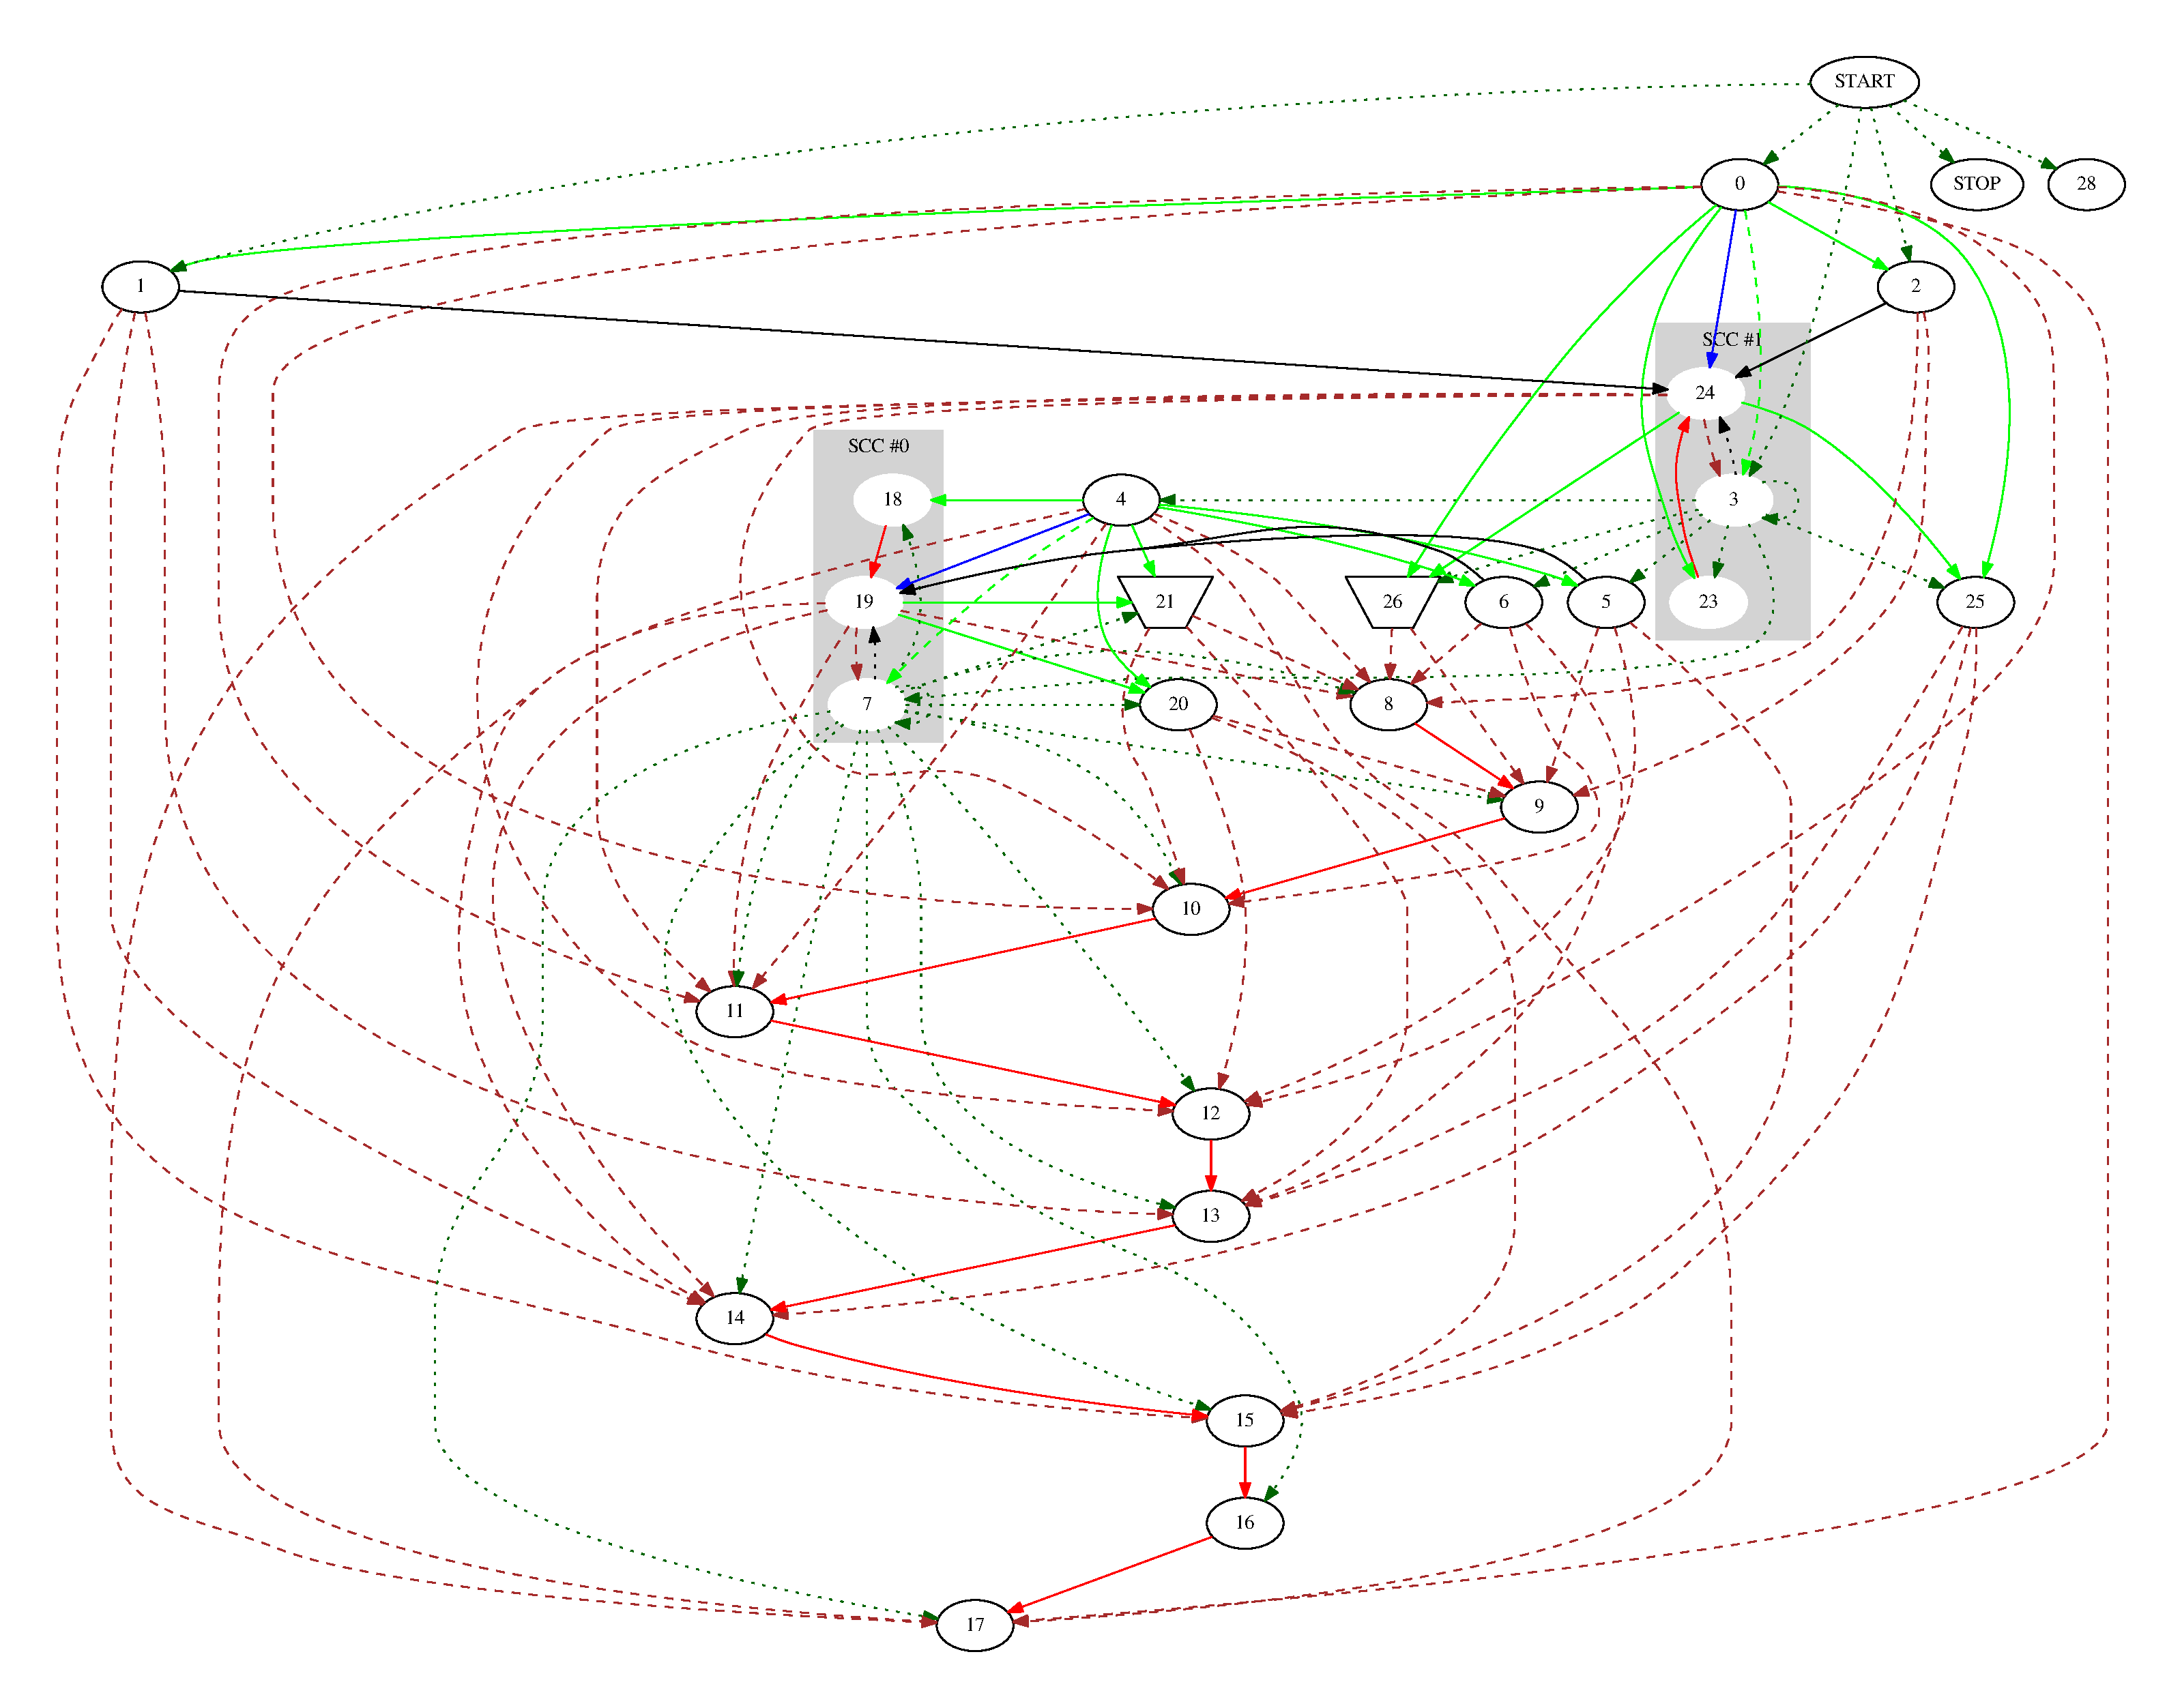
\includegraphics[width=\textwidth]{imm/tessa/PDGscc.pdf} 	\caption{
  	} 
  	\label{pdg}
  \end{figure}
The instruction in the SCC (Strongly Connected Components), shown as gray box, have to be performed sequentially in the same core, while the instructions linked in red lines (strong data dependencies) have can be performed sequentially in pipeline. The instructions in dot red line shows a weak data dependencies.